\begin{frame}[fragile]{5.1 Vetores: elementos e capacidade}
Um vetor reúne elementos do mesmo tipo em posições consecutivas.
\begin{lstlisting}
int temperaturas[5] = {26, 28, 30, 32, 34};
\end{lstlisting}
\begin{center}
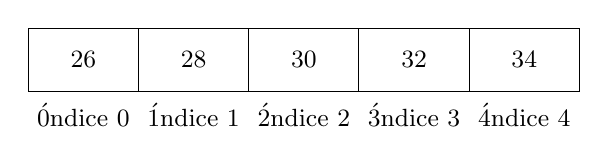
\begin{tikzpicture}[every node/.style={font=\small}]
\foreach \i/\v in {0/26,1/28,2/30,3/32,4/34} {
  \node[draw,minimum width=1.4cm,minimum height=0.8cm] at (\i*1.4,0) {\v};
  \node at (\i*1.4,-0.7) {índice \i};
}
\end{tikzpicture}
\end{center}
\begin{itemize}
\item Capacidade: cinco elementos do tipo \texttt{int}.
\item Primeiro índice: 0; último índice válido: 4.
\item \texttt{temperaturas[2]} contém 30, o terceiro elemento.
\end{itemize}
\end{frame}
